\documentclass[twocolumn,english,notitlepage]{article}  
\usepackage[margin=2cm]{geometry}

% \setlength{\parindent}{0pt} % no indents

\usepackage{overhead} % Overhead is in a separate file

\title{Studying the Efficiency of the Variational Quantum Eigensolver on the Lipkin-Meshkov-Glick Model using Quantum Machine Learning}
\author{Bendik Selvaag-Hagen, Håkon Kvernmoen}

\date{\centerline{\today}}

\begin{document}

\twocolumn[
    \begin{@twocolumnfalse}
        \maketitle
        \centerline{\text{Github:\space\space \url{https://github.com/hkve/Lipkin-Model-FYS5419/}}}
        \centerline{\space}
        \begin{abstract}
        A Quantum Mechanical System has a Hamiltonian which takes the system and computes its eigenvalues, corresponding to the systems energies. This is an efficient way of computing the energy of a system, but is computationally hard given an complicated initial state to which one needs to find the lowest energy. This problem is classically solved either by the diagonalization of the Hamiltonian or by the Variational Method. The latter has a numerical application used in Quantum Computing called the Variational Quantum Eigensolver (VQE). Applying the VQE to a simple  2x2 Hamiltonian with a interaction and non-interaction part on one state, we achieve accurately to recreate the analytical solution from the diagonalization with varying interaction strength. Expanding the model to two qubits, the entanglement entropy of the two states is found to increase with increased interaction strength. The diagonalized Hamiltonian still correspond sufficiently to the VQE on the system. Furthermore applying the VQE to the Lipkin-Meshkov-Glick model it is far superior to that of Hartree-Fock and Random Phase Approximation. VQE is deemed to be an accurate approximation to the diagonalized Hamiltonian of the Lipkin model, with no visual deviances for a two qubit system.
        \end{abstract}
    \end{@twocolumnfalse}
]

\tableofcontents

\section{Introduction}
\section{Introduction (men antagelig alt for basic)}
Quantum Mechanics (QM) is fundamentally hard, seeing as it has intrinsic uncertainties within, proclaimed by fundamental quantum theorems such as the Heisenberg Uncertainty Principle. Particles at such minuscule scales are not defined through classical physics, but as waves and wave-functions. To physically interpret the position and momentum of said particles need to be assessed as probability distributions. Thus it is manifestly encoded in the fabric of QM that it contains a certain amount of probabilistic features inherently in the fact that particles can not be expressed classically, but rather as states which develop. 
\newline\newline
For a Quantum Computer (QC) to be stern and act according to the probabilistic nature of the QM realm, we need to encode each bit as a state. This requires a short introduction to Classical Computing (CC). Here, the foundation of a circuit is a rigid state, 0 or 1, which can be altered, but which remain unaltered without external signals. One can operate on these bits, often system of bits, with gates such as OR and AND, and a plethora of more operations, which creates an outcome based on whether your selection of bits are in a state 0 or 1. 
\newline\newline
Comparing this CC to a QC, the encoding is still for QC bound by having bits of values 0 or 1, although here the similarities end. Each quantum state will in an ideal world not diverge from its original value, but seeing at it is probabilistic, it will evolve and fluctuate between 0 and 1. For the sake of simplicity, we assume and ideal world where it remains in its encoded state. Each operation on the state or the collection of states has to be unitary, to retain reversibility. And most importantly, states can be in a superposition of 0 and 1, making the outcome reliant on lots of runs, seeing as the outcome is probabilistic. Two or more states can also be entangled, in a manner at which predicts with certainty the outcome of the first bit, based on the measurement on the second. These properties makes QC capable of, through different encoding and operating schemes, to solve some problems within computing better than its classical counterpart. 
\newline\newline
\textbf{This is the part where I introduce our hamiltonian problem.}
\subsection{Dårlig intro som kan taes med om vi er kritisk}
There are lots of questions within the realm of Quantum Computing (QC). Most of them are never answered, due to, more or less, our inability to discover the true nature of quantum mechanics, and our ability to predict future breakthroughs. Questions about the feasibility of applying QC to problems ranging from NP-hard classical problems to distinct quantum problems, such as computing energies of a quantum state are perpetually conjectured, but alas, the state of current QC schemes are lacking. This paper will in brief answer none of these questions, but apply the foundations of QC to further speculate.


\section{Quantum Computing}
\subsection{Notation}
The basic building block of a QC is the \textit{qbit}. Resembling the binary representation in CC, the qbit is defined as a two-level system. In the canonical/standard/Pauli basis, we express the basis states as
\begin{align*}
    \ket{0} = \begin{pmatrix}
        1 \\
        0
    \end{pmatrix}, \ket{1} = \begin{pmatrix}
        0 \\ 
        1
    \end{pmatrix}.
\end{align*}
Despite the similarity to bits, a qbit is allowed to be in a superposition of the two basis states, meaning that 
\begin{align*}
    \ket{\psi} = c_0 \ket{0} + c_1 \ket{1}, \hspace{20px} c_0,c_1 \in \mathbb{C}
\end{align*}
is also a valid qbit, constrained to normalization $|c_0|^2 + |c_1|^2 = 1$. The modulus of the coefficients $c_0,c_1$ are through the Born rule interred as the point probability of measuring basis state $\ket{0}$ and $\ket{1}$ respectively, mirroring probability vectors. However, the qbits $\set{\ket{\psi}_i}$ are expressed through the coefficients $\set{c_i}$ and not their modulus, allowing both negative and complex values, resulting in the possibility for both constructive and destructive interference when added together.

We are however not only limited to a single qbit. Composite systems of two-level qbits can be created, mathematically expressed as tensor products between states. Considering the Pauli basis $\set{\ket{0},\ket{1}}$, we can create a new basis $\set{\ket{00},\ket{01},\ket{10},\ket{11}}$ through the operation
\begin{align}
    \ket{ij} = \ket{i} \otimes \ket{j} \hspace{20px} i,j=0,1. \label[eq]{eq:theo:pauli_matricies_definition}
\end{align}
The above procedure can be repeated for more than two qbits. In the realm of QC, the most important operators are the Pauli matrices, often referred to the $X,Y$ and $Z$ \textit{gates} 
\begin{align}
    X = \begin{pmatrix}
        0 & 1 \\
        1 & 0
    \end{pmatrix}, Y = \begin{pmatrix}
        0 & -i \\
        i & 0
    \end{pmatrix}, Z = \begin{pmatrix}
        1 & 0 \\
        0 & -1
    \end{pmatrix}
\end{align}
Just as with qbits, we can through the tensor product compose operators acting on multiple qbits. To avoid potential confusion between multiple operators being applied and composite operators, a subscript on these operators will be added. For instance, a three qbit operator can be constructed as
\begin{align}
    X_1 Z_3 = X \otimes I \otimes Z 
\end{align} 
Where $I$ is the $2 \times 2$ identity matrix. Here $X_1 Z_3$ applied to a three qbit state applies $X$ to the first qbit, does nothing with the second and applies $Z$ on the third.
% \begin{align*}
%     \ket{+} = \frac{1}{\sqrt{2}} (\ket{0} + \ket{1}) \\ 
%     \ket{-} = \frac{1}{\sqrt{2}} (\ket{0} - \ket{1})
% \end{align*}

\subsection{Basics of Quantum Computing}
In the introduction, vague outlines of the functionality of QC is presented. In this section, the circuits and representation will be presented with a elementary example of circuits and states. A Greenberger-Horne-Zeilinger(GHZ) State is a  fully entangled set of three or more quantum bits, or qbits. For two qbits, this is called a Bell-state. It can be encoded by applying a Haddamard gate to the primary gate, and CNOT gates to the subsequent. In matrix representation these operations are
\begin{equation}
    H = \begin{pmatrix}
    1 & 1 \\
    1 & -1 
    \end{pmatrix} \qquad 
    CNOT = \begin{pmatrix}
    1 & 0 & 0 & 0 \\
    0 & 1 & 0 & 0 \\
    0 & 0 & 0 & 1 \\
    0 & 0 & 1 & 0 
    \end{pmatrix} \label[eq]{eq:theo:CNOT_Hadamard}
\end{equation}
\begin{figure}
    \centering
    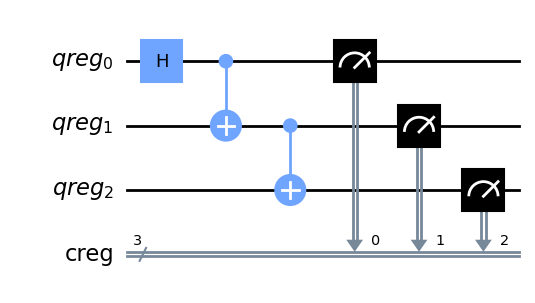
\includegraphics[width=\linewidth]{figs/GHZ.png}
    \caption{The circuit needed to initialize the GHZ state for three qubits.}
    \label{fig:GHZ_circ}
\end{figure}
Hadamard gates changes the basis of the gate between Pauli Z and Pauli X basis. CNOT changes the affected gate, based on the state of the control state. Visually, in a circuit, this can be presented as shown in Fig(\ref{fig:GHZ_circ}).
The result is a full entanglement, as seen in Fig(\ref{fig:qshpere}), where the outcome of any measurement on any qbit, will ascertain the outcome of all other measurements, as shown in Fig(\ref{fig:GHZ_measure}).
\begin{figure}[H]
    \centering
    \begin{subfigure}{0.48\textwidth}
        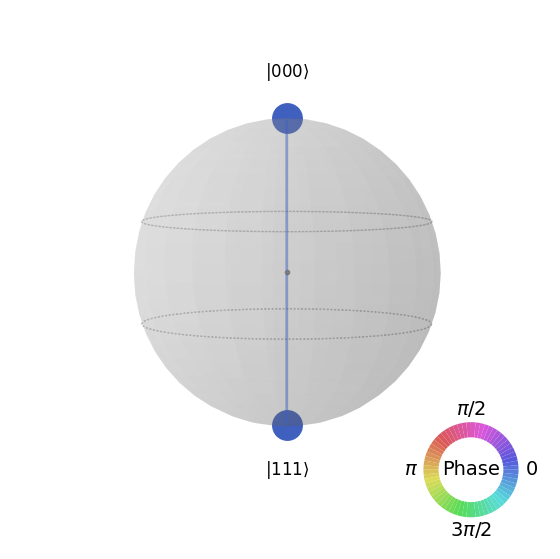
\includegraphics[width=\textwidth]{figs/GHZ qsphere.png}
        \caption{The Bloch-sphere representation of the GHZ state, given three qubits. It is strictly entangled, by their parallell nature.}
        \label{fig:qshpere}
    \end{subfigure}
    \hfill
    \begin{subfigure}{0.48\textwidth}
        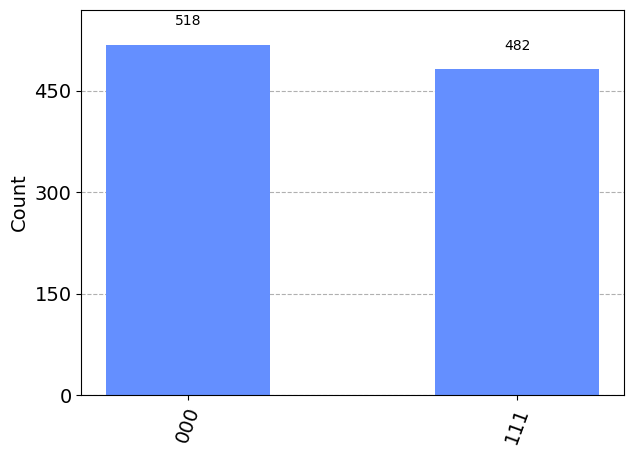
\includegraphics[width=\textwidth]{figs/GHZ Counts.png}
        \caption{The outcome of measurements of the GHZ state with three qubits.}
        \label{fig:GHZ_measure}
    \end{subfigure}
\end{figure}
Another important set of gates are the \textit{rotation operators} $R_x, R_y$ and $R_z$. By application to a qbit, we can reach any point on the Bloch sphere by usage of all three once. They are expressed as
\begin{align}
    \begin{split}
        R_x(\theta) &= \exp{-iX\theta/2} = \begin{pmatrix}
            \cos(\theta/2) & -i\sin(\theta/2) \\
            -i\sin(\theta/2) & \cos(\theta/2)
        \end{pmatrix}, \\
        R_y(\theta) &= \exp{-iY\theta/2} = \begin{pmatrix}
            \cos(\theta/2) & -\sin(\theta/2) \\
            -\sin(\theta/2) & \cos(\theta/2)
        \end{pmatrix}, \\
        R_z(\theta) &= \exp{-iZ\theta/2} = \begin{pmatrix}
            \exp{-i\theta/2} & 0 \\
            0 & \exp{i\theta/2}
        \end{pmatrix}
    \end{split}\label[eq]{eq:theo:bloch_rotations}
\end{align}
with all having a period of $4\pi$.

\subsection{Pauli Encoding Hamiltonians}
To apply a specific system to VQE, the Hamiltonian must be re-written in terms of a sum of \textit{Pauli strings}. Considering the identity $I$ and the three Pauli matrices $X, Y, Z$, we construct a specific term as a tensor product of these $P_i$. For an $n$-qubit system, we require $n-1$ tensor products. Combined with a weight $w_i$, the Hamiltonian must be written in the from
\begin{align}
    H = \sum_i w_i P_i \label[eq]{eq:theo:pauli_encoding_general}
\end{align}
For a general two-body Hamiltonian, this task can serve challenging. Many schemes exists for this purpose, such as the Jordan-Wigner transformation \citep{steudtnerMethodsSimulateFermions2019}. For the Lipkin model, an easier approach is available since the Hamiltonian can be written as products of the number and spin operators.


\subsection{Variational Quantum Eigensolver}
In this section we will briefly remind the reader of some key aspects of the variational method, followed by an outline on how observable values can be calculated using a QC. 

\subsubsection{Brief Remainder of the Variational Method}
The Rayleigh-Ritz VM states that for a given Hamiltonian $H$, the expectation value of a \textit{trial state} or \textit{ansatz} $\ket{A}$ puts a lower bound on the ground state energy $E_0$.
\begin{equation}
    \frac{\bra{A}H\ket{A}}{\ip{A}} \geq E_0
\end{equation}
The ansatz is typically chosen to be a parameterized superposition of basis states that can be varied to improve the energy estimate, $\ket{A}\equiv \ket{A(\boldsymbol{\theta})}$ where $\boldsymbol{\theta} = (\theta_1, \ldots, \theta_M)$ are the $M$ optimization parameters.

This is a crucial method in many-body theory, where good estimates of ground state energies are crucial due to the lack of analytical solutions. In contrast to perturbation theory, the VM will not give too small ground state energies, assuming that the ansatz has some overlap with the true ground state. The VM machinery form the basis of the VQE. 

\subsubsection{Algorithm}
We wish to apply the VM to estimate the ground state energy of a Hamiltonian on a quantum computer. To have any flexibility in the ansatz $\ket{A}$, we need to allow for parametrization. The most common approach is the so-called $RY$ ansatz, where we apply chained operations of rotating around the $y$-axis (\cref{eq:theo:bloch_rotations}) by $\boldsymbol{\theta} = (\theta_1,\ldots,\theta_Q)$ of the Bloch sphere and CNOT operations (\cref{eq:theo:CNOT_Hadamard}). Applications of $y$ rotations specifically ensures that our coefficients always remain real, which often is satisfactory when dealing with many-body systems. \comment{Hadde det gått å laget et plot som \url{https://i.stack.imgur.com/740xL.png} i qiskit?}

After the ansatz construction has been performed, the Hamiltonian must be applied. As discussed, the Hamiltonian must be written in terms of Pauli strings such that it is expressible as \cref{eq:theo:pauli_encoding_general}. To obtain the expectation value of the ground state energy, one can measure the expectation value of each Pauli string,

\begin{align*}
    E(\boldsymbol{\theta}) = \sum_i w_i\bra{A(\boldsymbol{\theta})} P_i \ket{A(\boldsymbol{\theta})} \equiv \sum_i w_i f_i,
\end{align*}
where $f_i$ is the expectation value of the Pauli string $i$. This is estimated statistically by considering measurements in the appropriate basis of the operator in the Pauli string. If the $P_i \supseteq Z_1$ we simply subtract the $0$ and $1$ outcomes of the first qbit, averaged over all measurements. If however we also have $P_i \supseteq X_2$, the second qbits measurement must be taken along the $x$-axis\footnote{To do this, we must must transform the qbit from the Pauli $z$-basis to the Pauli $x$-basis by application of a Hadamard gate.}. This with $N_0$ and $N_1$ as the number of $0$ and $1$ measurements respectively, we can estimate $f_i$ since 
\begin{align*}
    f_i = \lim_{N \to \infty} \frac{N_0 - N_1}{N},
\end{align*}
with $N$ as the number of shots (measurements). Therefor each Pauli string requires it own circuit, where multiple measurements of each string is required. Adding the results together with the corresponding weights, the ground state energy can be estimated. To optimize wrt. $\boldsymbol{\theta}$, a classical optimizer is often applied. Gradients are estimated using a simple finite difference approximation

\begin{align}
    \nabla_{\boldsymbol{\theta}} E(\boldsymbol{\theta}) \approx \frac{E(\boldsymbol{\theta} + \delta \boldsymbol{\theta})-E(\boldsymbol{\theta} - \delta \boldsymbol{\theta})}{2\delta \theta} ,
\end{align}
where $\delta \boldsymbol{\theta} = (\delta \theta, \ldots, \delta \theta)$. By updating the previous $\boldsymbol{\theta}$ values with some scalar times the negative of the gradient estimate, a new set of $\boldsymbol{\theta}$ values are obtained. The process is then repeated a finite amount of steps, where we hope to converge to the global minimum. A schematic of the procedure is presented in \cref{fig:VQE_scheme}

\noindent\rule{8.8cm}{0.8pt}
The Variational Quantum Eigensolver(VQE) takes on applying the Variational Principle, described above, minimizing the energy of 
\begin{equation}\label{VQE}
    E_{temp} = \frac{\bra{a}\boldsymbol{H}\ket{a}}{\braket{a}}
\end{equation}
with regards to altering the state $\ket{a}$. This is achieved by applying an ansatz to the initial state, in order to get an output eigenvalue, which further can be minimized. The ansatz takes \textit{n} Quantum Bits (qbits) and \textit{n} free parameters, $\theta_i$. The goal of the algorithm is to alter the parameters $\theta_i$ in order to achieve the optimal the minimal energy of the system, as computed in Eq. (\ref{VQE}). A schematic of the process is shown in Fig(\ref{fig:VQE_scheme}). The ansatz conjectured by Hlatshwayo et al. \cite{} is shown in Fig. (\ref{fig:ansatz}). 
\begin{figure}[H]
    \centering
    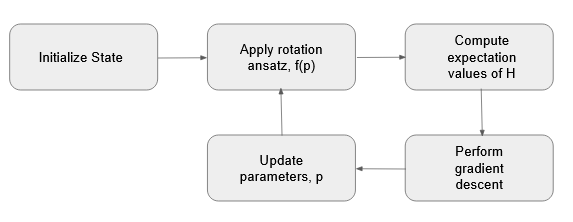
\includegraphics[width=\linewidth]{figs/VQE.PNG}
    \caption{A schematic of the process of Variational Quantum Eigensolvers.}
    \label[fig]{fig:VQE_scheme}
\end{figure}
\begin{figure}[H]
    \centering
    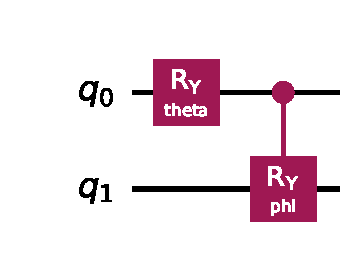
\includegraphics[width=\linewidth]{figs/ansatz.pdf}
    \caption{The ansatz for the VQE scheme applied for N = 4. }
    \label[fig]{fig:ansatz}
\end{figure}

\section{Quantum Systems}
This section will introduce the three relevant systems for this work. Initially we will look at two `toy models`, being $2\times2$ and $4 \times 4$ real Hamiltonians with arbitrary entries. Lastly the Lipkin model will be used, showing many of the key features of many-body systems while still being analytically solvable.   

\subsection{$H \in \mathbb{R}^2$ Hamiltonian}
As an initial test, we will consider a simply $2\times 2$ real Hamiltonian consistend of a diagonal part $H_0$ and off-diagonal part $H_I$, playing the roles of a non-interactive one-body and interactive two-body part respectively. Defined through their matrix elements, we express them in the Pauli basis $\set{\ket{0},\ket{1}}$

\begin{align}
    \begin{split} \label[eq]{eq:theo:2times2_hamiltonian}
        H &= H_0 + H_I \\
        H_0 = \begin{pmatrix}
            E_1 & 0 \\
            0 & E_2
        \end{pmatrix}&, \hspace{20px}
        H_I = \lambda \begin{pmatrix}
            V_{11} & V_{12} \\
            V_{21} & V_{22}
        \end{pmatrix}
    \end{split}
\end{align}
Where $\lambda \in [0,1]$ is a coupling constant parameterizing the strength of the interaction. 

\subsection{$H \in \mathbb{R}^4$ Hamiltonian}
We now move on to a slightly larger system, defined as a $4 \times 4$ real Hamiltonian. This can be viewed as two  composite systems where each system is a two-level system. In the product basis $\set{\ket{00},\ket{01},\ket{10},\ket{11}}$ we define the one-body part as 
\begin{align}
    H_0 \ket{ij} = \epsilon_{ij}\ket{ij}, \label[eq]{eq:theo:4times4_diagonal_hamiltonian}
\end{align}
with a two-body interaction defined using Pauli matricies
\begin{align}
    \begin{split} \label[eq]{eq:theo:4times4_interaction}
        H_I &= H_x X \otimes X + H_z Z \otimes Z \\
        &= \begin{pmatrix}
            H_z & 0 & 0 & H_z \\
            0 & - H_z & H_x & 0 \\
            0 & H_x & - H_z & 0 \\
            H_x & 0 & 0 & H_z
        \end{pmatrix}
    \end{split}
\end{align}
Where $H_x$ and $H_y$ are couplings playing the same role as $\lambda$.

\subsection{Lipkin Model}
For larger many-body systems, the introduction of the occupation representation is common. The creation of a state $p$ is represented by the operator $\crt{p}$, while annihilation $\ani{p}$. Since we are dealing with fermions, the creation and annihilation operators follow the canonical anitcommutation relations
\begin{align}
    \set{\crt{p},\crt{q}} = \set{\ani{p},\ani{q}} = 0, \hspace{10px}\set{\crt{p},\ani{q}} = \delta_{pq}. 
    \label[eq]{eq:theo:car_algebra}
\end{align}
The Lipkin model \citep{lipkinValidityManybodyApproximation1965} for a $N$ fermion system consists of two energy levels $\sigma \in \set{\pm 1}$, each having a degeneracy of $N$. Resembling fermionic half integer spin, the two levels contributes energetically $\pm \frac{1}{2}\epsilon$ for each particle. Additionally, we label the different states in each degenerate level by $p = 1, \ldots N$ \footnote{This removes the spin quantum number from $p$, which commonly is included.}. The Lipkin Hamiltonian can be written using creation and annihilation operators as 
\begin{align}
    \begin{split}\label[eq]{eq:theo:lipkin_second_quant_hamiltonian}
    H &= H_0 + H_1 + H_2, \\
    H_0 &= \frac{1}{2}\epsilon \sum_{pq} \sigma \crt{p\sigma} \ani{p\sigma}, \\
    H_1 &= \frac{1}{2}V \sum_{pp'\sigma} \crt{p\sigma}\crt{p'\sigma}\ani{p'\bar{\sigma}}\ani{p\bar{\sigma}}, \\
    H_2 &= \frac{1}{2}W \sum_{pp'\sigma} \crt{p\sigma} \crt{p'\bar{\sigma}} \ani{p'\sigma} \ani{p\bar{\sigma}}.
    \end{split}
\end{align}
With $\bar{\sigma} = -\sigma$. $H_0$ is a diagonal single particle operator giving a contribution based on occupancy in the different levels. $H_1$ and $H_2$ are two-body operators moving pairs of particles between levels and exchanging particles between levels (spin-exchange) respectively. The strengths of these effects are parameterized by the couplings $V$ and $W$. By defining the \textit{quasi-spin} operators $J_\pm , J_z, J^2$ in addition to the number operator $N$ as 
\begin{align}
    \begin{split}\label[eq]{eq:theo:quasi_spin_definitions}
        J_\pm = \sum_p \crt{p\pm}\ani{p\mp} \\
        J_z = \frac{1}{2}\sum_{p\sigma} \sigma \crt{p\sigma} \ani{p\sigma} \\
        J^2 = J_+ J_- + J_z^2 - J_z \\
        N = \sum_{p\sigma} \crt{p\sigma} \ani{p\sigma}
    \end{split}
\end{align}
we can rewrite the Lipkin Hamiltonian from \cref{eq:theo:lipkin_second_quant_hamiltonian} using these
\begin{align}
    \begin{split} \label[eq]{eq:theo:lipkin_quasispin_hamiltonian}
        H_0 &= \epsilon J_z, \\
        H_1 &= \frac{1}{2}V (J_+^2 + J_-^2), \\
        H_2 &= \frac{1}{2}W ( \set{J_+ , J_- } - N ),
    \end{split}
\end{align}
These quasi spin operators obey the normal spin commutator relations
\begin{align*}
    &\commutator{J_z}{J_\pm} = \pm J_\pm, 
    &\commutator{J_+}{J_-} = 2 J_z, \\
    &\commutator{J^2}{J_\pm} = 0,
    &\commutator{J^2}{J_z} = 0,
\end{align*}
in addition to commuting with the number operator
\begin{align*}
    \commutator{N}{J_z} = \commutator{N}{J_\pm} = \commutator{N}{J^2} = 0.
\end{align*}
Using these relations we can show that the Hamiltonian (a product of quasi spin operators and the number operator) also commutes with  $J^2$, that is $\commutator{H}{J^2}=0$. Therefor $H$ and $J^2$ have shared eigenbasis, with $J$ being a `good` quantum number.

Using spin-eigenstates as the Hamiltonian basis, we define states through the normal approach $\ket{J,J_z}$ with $J$ and $ J_z$ as spin and spin-projections respectively. The states $J_z = \pm J$ are the easiest to construct, corresponding to a single level being completely filled. States in between can then be found using the quasi-spin ladder operators following

\begin{align}
    J_\pm \ket{J,J_z} &= \sqrt{J(J+1)-J_z (J_z \pm 1)} \ket{J,J_z \pm 1}. \label[eq]{eq:theo:ladder_operations}
\end{align}
Using this basis for the quasi-spin Hamiltonian from \cref{eq:theo:lipkin_quasispin_hamiltonian}, the explicit matrix $H_{J_z,J'_z} = \bra{J,J_z} H \ket{J,J_z'}$ can be constructed.

\comment{Rekkefølgen følger $\bra{J,-J} H \ket{J, -J}$ som $H_{0,0}$, motsatt av artikkelen}

\comment{Her med $W$, tror Morten har surra litt og her brukt hamiltonen $H = H_0 - H_1 - H_2$ samt uten $N$ operator}
\begin{align}
    H = \begin{pmatrix}
        -(\epsilon-W) & 0 & -V \\
        0 & -2W & 0 \\
        -V & 0 & \epsilon - W
    \end{pmatrix}
\end{align}

\comment{med $H = H_0 + H_1 + H_2$ og $N$ inkludert}
\begin{align}
    H = \begin{pmatrix}
        -\epsilon & 0 & V \\
        0 & W & 0 \\
        V & 0 & \epsilon
    \end{pmatrix}
\end{align}

\comment{$J=2$ er good med $H = H_0 + H_1 + H_2$}
\begin{align}
    H = \begin{pmatrix}
        -2\epsilon & 0  & \sqrt{6}V &0 &0 \\
        0 & -\epsilon + 3W & 0 & 3V & 0 \\
        \sqrt{6}V & 0 & 4W & 0 & \sqrt{6}V \\
        0 & 3V & 0 & \epsilon + 3W & 0 \\
        0 & 0 & \sqrt{6}V & 0 & 2\epsilon
    \end{pmatrix}
\end{align}

\subsection{Encodings}
\subsubsection{Toy Hamiltonians}
Show explicit $2\times 2$ and $4\times 4$ expressions with Pauli matrices.
\subsubsection{Lipkin Model}
Using the level mapping \comment{introduce the mappings?}, the spin operators from \cref{eq:theo:quasi_spin_definitions} can be written using their one-body counterparts as 
\begin{align}
    J_z = \sum_{i}^{N} \spinsmall{z}{i} \hspace{20px} J_\pm = \sum_i^N \spinsmall{\pm}{i} = \sum_i^N (\spinsmall{x}{i}\pm i\spinsmall{y}{i}) \label[eq]{eq:met:quasispin_to_onebody_mapping}
\end{align}
with $N$ being the number of particles. Additionally, since we have spin-$\sfrac{1}{2}$ fermions, the mapping to Pauli matrices follow
\begin{align}
    \spinsmall{x}{i} = \frac{1}{2}X_i,\hspace{20px}\spinsmall{y}{i} = \frac{1}{2}Y_i,\hspace{20px}\spinsmall{z}{i} = \frac{1}{2}Z_i. \label[eq]{eq:met:onebody_to_pauli_mapping}
\end{align}
As shown in \cref{sec:app:pauliencoding_detailed}, \cref{eq:theo:lipkin_quasispin_hamiltonian} can be expressed as
\begin{align}
    \begin{split}\label[eq]{eq:met:lipkin_pauli_hamiltonian}
        H_0 &= \frac{\epsilon}{2}\sum_{p}Z_p  \\
        H_1 &= \frac{1}{2}V \sum_{p < q} X_p X_q - Y_p Y_q \\
        H_2 &= \frac{1}{2}W \sum_{p < q} \pclosed{ X_p X_q + Y_p Y_q } 
    \end{split}
\end{align}


\section{Results}
\subsection{Toy Models}

The energy eigenstates and $\set{\ket{0},\ket{1}}$ coefficients for the $H \in \mathbb{R}^2$ Hamiltonian as a function of interaction strength $\lambda$ is shown in figure \cref{fig:res:changing_character}. Despite having two free parameters $C_0,C_1$ they are constrained through normalization.  
\begin{figure}[H]
    \centering
    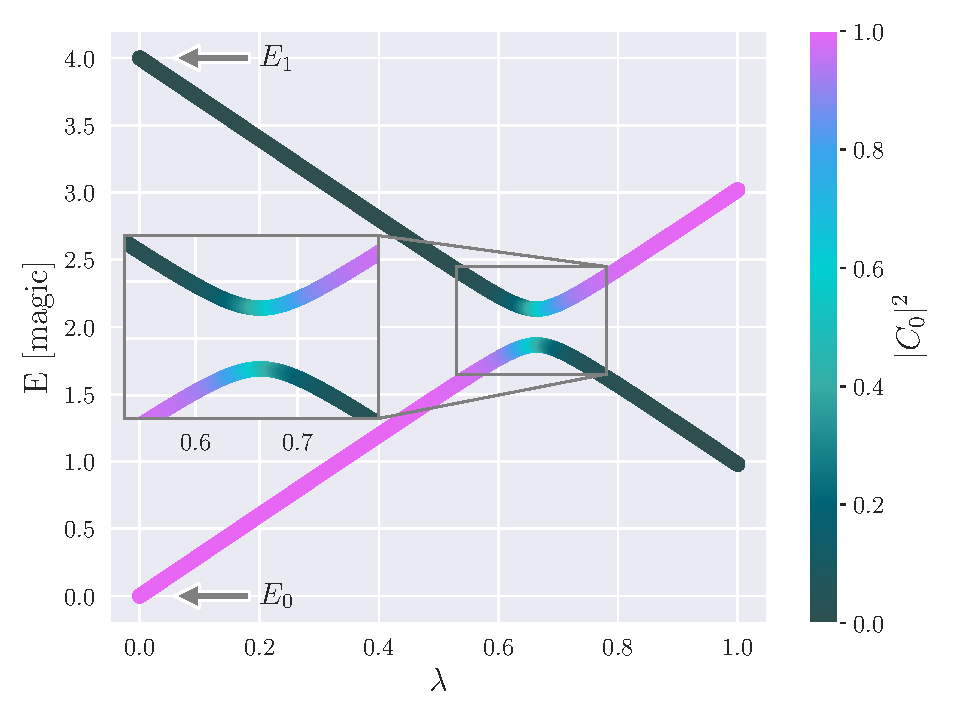
\includegraphics[width=\linewidth]{figs/chaning_character.pdf}
    \caption{Energy eigenstates and coefficients of $2 \times 2$ Hamiltonian when varying the interaction strength $\lambda \in [0,1]$. Calculations done using exact diagonalization.}
    \label[fig]{fig:res:changing_character}
\end{figure}

The entropy of entanglement in the case of the of the Hamiltonian consisting of a interacting and non-interacting between the two states, is presented in Fig. (\ref{fig:entropy}). It is apparent that the entropy of entanglement increases as the connection strength increases. 

\begin{figure}
    \centering
    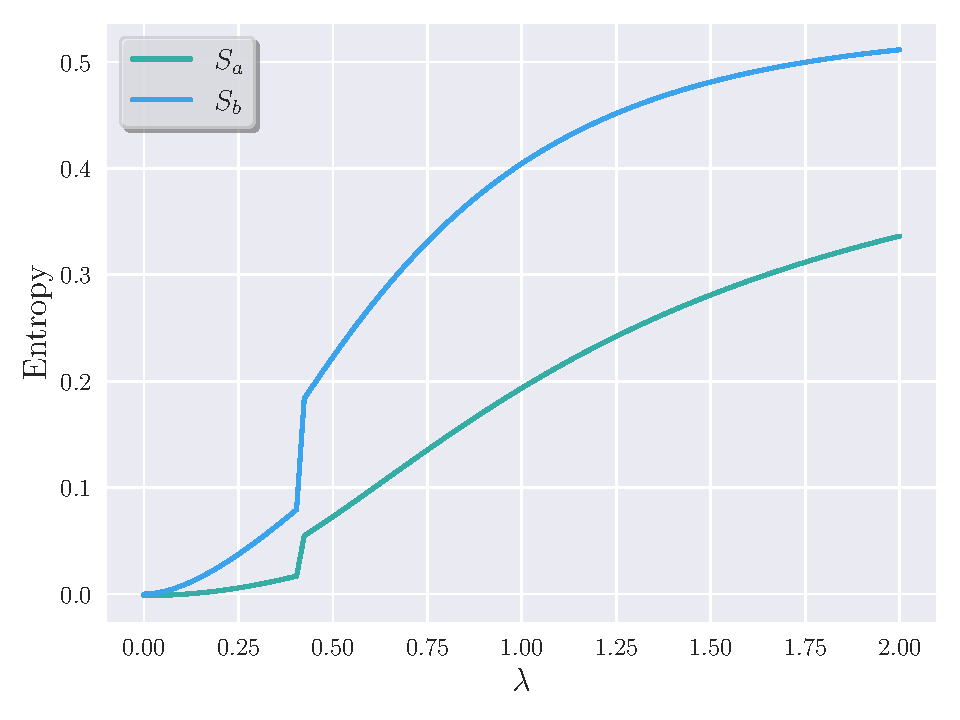
\includegraphics[scale=0.4]{figs/Entropy.pdf}
    \caption{Caption}
    \label{fig:entropy}
\end{figure}

\subsection{Lipkin Model}

\begin{figure}[H]
    \centering
    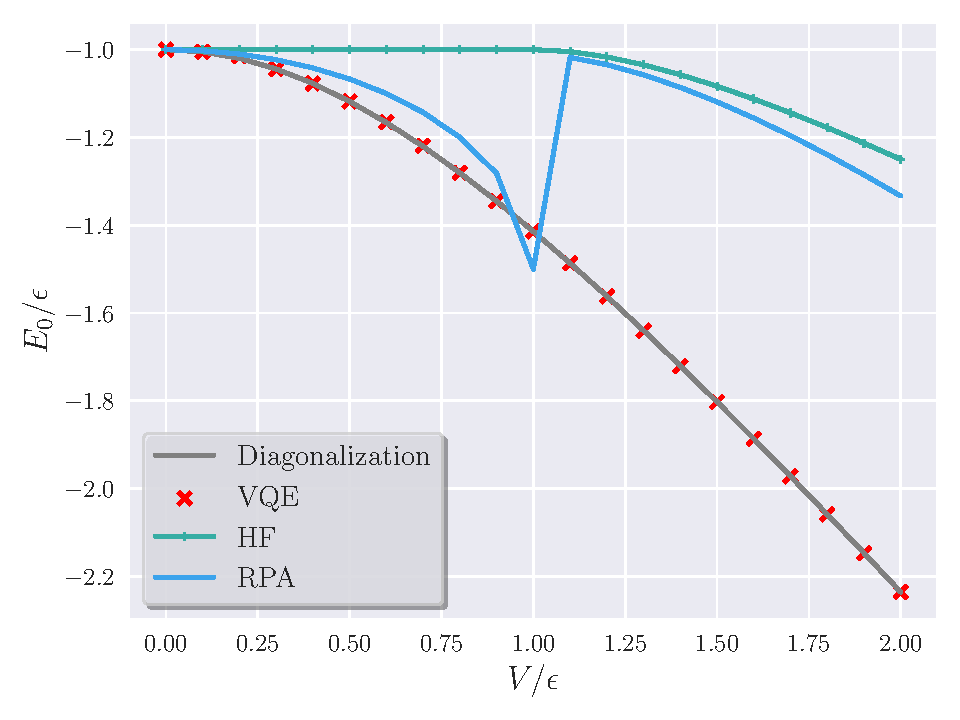
\includegraphics[width=\linewidth]{figs/N2_lipkin_vary_V.pdf}
    \caption{Ground state values for the Lipkin model for $N=2$ particles with $W = 0$ as a function of $V/\epsilon$. Calculations were done using exact diagonalization, VQE, in addition to closed form HF and RPA expressions.}
    \label[fig]{fig:res:Lipkin_N2_vary_v}
\end{figure}

\begin{figure}[H]
    \centering
    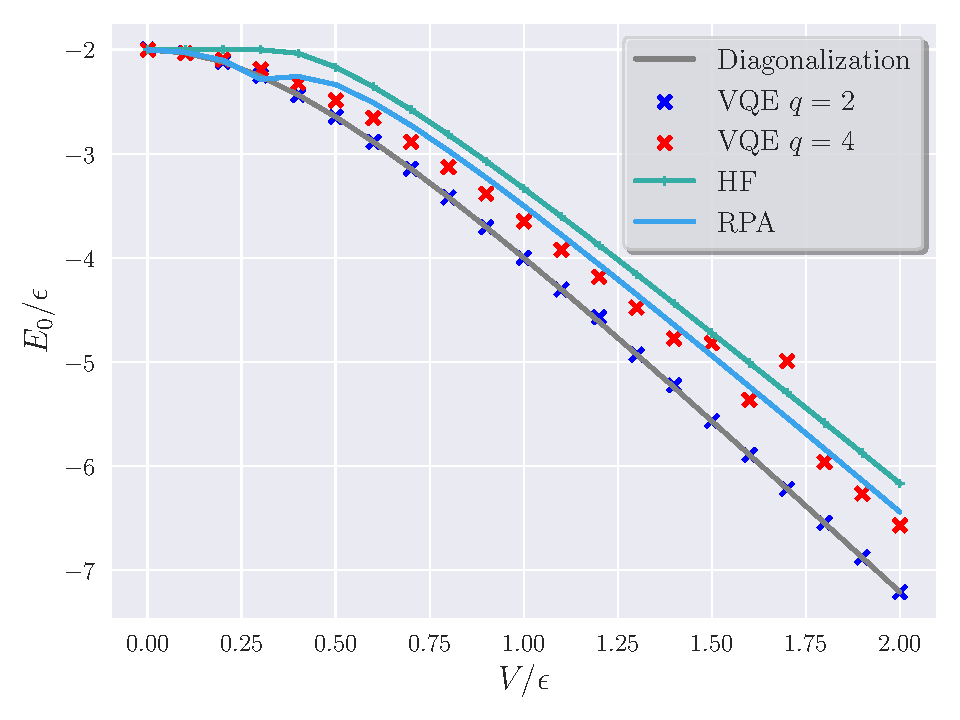
\includegraphics[width=\linewidth]{figs/N4_lipkin_vary_V.pdf}
    \caption{Ground state values for the Lipkin model for $N=4$ particles with $W = 0$ as a function of $V/\epsilon$. Calculations were done using exact diagonalization, VQE, in addition to closed form HF and RPA expressions.}
    \label[fig]{fig:res:Lipkin_N4_vary_v}
\end{figure}


\begin{figure}[H]
    \centering
    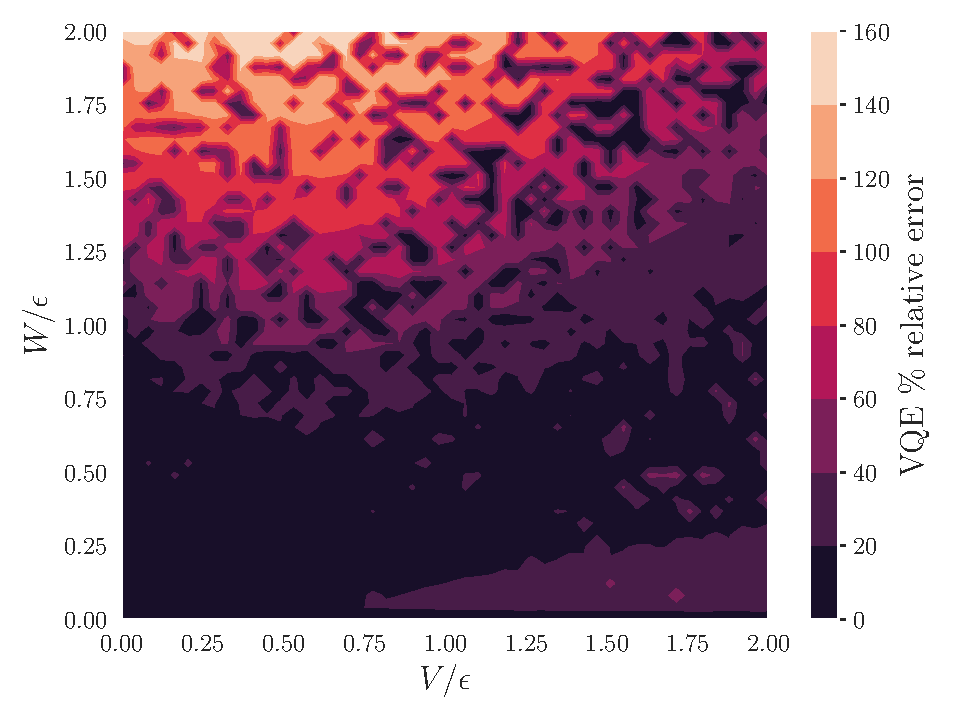
\includegraphics[width=\linewidth]{figs/50pts_vw_grid.pdf}
    \caption{Ground state values for the Lipkin model for $N=4$ particles with $W = 0$ as a function of $V/\epsilon$. Calculations were done using exact diagonalization, VQE, in addition to closed form HF and RPA expressions.}
    \label[fig]{fig:res:lipkin_N4_vw_grid}
\end{figure}


\section{Discussion}
\subsection{Toy models}
Going back to \cref{fig:res:changing_character} we see the classical example of level crossing in two-level systems. The phenomenon gets its name because in a plot of energy versus interaction strength, the energy levels appear to cross or avoid crossing each other, depending on the specific parameters and interactions involved, as seen. Taking a look at the coefficients, we see that for small interaction strengths $\lambda$, the ground state and excited state are almost purely dominated by $\ket{0}$ and $\ket{1}$ respectively. Increasing $\lambda$, the domination is less and less present. This continues until we reach $\lambda = 2/3$, where the ground state energy is maximal and excitation energy minimal. Moving past  $\lambda = 2/3$ results in the ground state being dominated by $\ket{1}$ and the excited state by $\ket{0}$, meaning that the states has change or swapped character.


\begin{figure}
    \centering
    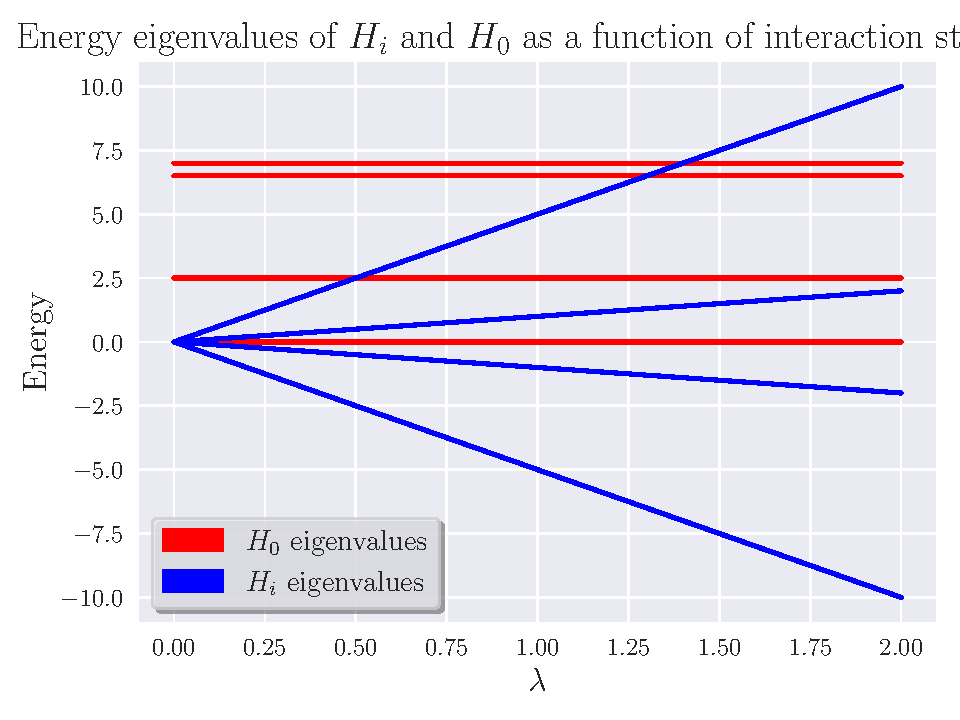
\includegraphics[scale=0.4]{figs/Eig_lmd.pdf}
    \caption{Caption}
    \label{fig:eig_lmd}
\end{figure}
The entropy in Fig. (\ref{fig:entropy}) has an initial contribution which increases slower, before taking a leap for a connection strength of $\lambda \approx 0.4$. This is probably a jump corresponding to a system being slightly interacting into being entangled. The entanglement further increases before converging around $\lambda \approx 1.3$. Studying Fig(\ref{fig:eig_lmd} Overlap) we can extract some information, seeing as the first jump is correlated with the eigenvalues of the interaction Hamiltonian overcoming the second lowest eigenvalues. The convergence can be interpreted as the interaction energy overcoming the higher eigenvalues of the non-interaction Hamiltonian.
\newline\newline

The decision of the ansatz in Fig. (\ref{fig:ansatz}) seems a bit arbitrary, but is based on the ansatz in Hlatshwayo et al. (\cite{hlatshwayoSimulatingExcitedStates2022}). There could be possibilities in optimization by choosing a different ansatz. This would be a section of further research by delving into a review of VQE by Tilly et al. (\cite{VQE_review}). \newline 
Further research could look into other methods of optimization, other than the VQE algorithm, as it is a fairly simple model with restricted applicability. It could probably be extended to solving other optimization problems with minor tweaks or clever encoding. The Lipkin model is fairly limited when it comes to QC. This is a result of the angular momentum operators $j_+$ and $j_-$ are not unitary and thus not applicable to general QC. Thus other models could be further researched in order to not simplify the Hamiltonian by non-unitarity. These models become fairly complex quickly and involves heavier computational costs in order to construct and optimize. \comment{Mangler litt idé om fler ting å kunne ta opp her.} 

\subsection{Lipkin Model}
From \cref{fig:res:Lipkin_N2_vary_v} we see good agreement between diagonalization and VQE. There were little trouble with convergence and precise results were obtained after just 30 iterations. The variability between runs were also minuscule, except when running for less than 30 iterations. It is also clear that VQE beats both HF and RPA consistently for the range of interaction strengths. 

Moving on to the four particle case from \cref{fig:res:Lipkin_N4_vary_v}, the precision of the results decreases. The two qbit scheme making use of the $W=0$ symmetry still shows excellent agreement with the diagonalization, but the larger four qbit scheme performs worse. This was the case despite increasing the number of iterations to 1000. Still, the four qbit results outperformed both HF and RPA for all except two interaction strengths, but showed some variability in results across identical runs. We hypothesize multiple reasons for this. Firstly, the number of Pauli string from \cref{eq:met:lipkin_N4_dumb} is 16 compared to the encoding from \cref{eq:met:lipkin_N4_smart_hamiltonian} only containing 6. We are therefor reliant on good estimates of Pauli string expectation values for more terms. If one or more of these estimates are poor for one iteration, the gradient estimate or the energy evaluation itself could be erroneously, resulting in slower converge. Intertwined with this is the sice of the parameter space which is twice as large for the four qbit case. Optimization here is harder and could hinder the convergence of the VQE. The $RY$ ansatz could of course also be too naive, restricting to only real amplitudes. Various different approaches are present in the literature, for instance the popular Unitary Coupled Cluster \citep{peruzzoVariationalEigenvalueSolver2014} being one of the gold standards in quantum chemistry. 
The runtime also increased with more qbits as expected. This is a clear indication that spending time reducing the number of Pauli strings by considering the symmetries of the system at hand is a worthwhile task.

When lifting the $W=0$ restriction, such as we saw in \cref{fig:res:lipkin_N4_vw_grid_VQE}, the convergence trouble was more apparent. For low $W$ values, the VQE outperformed both HF and RPA from \cref{fig:res:lipkin_N4_vw_grid_HF} and \cref{fig:res:lipkin_N4_vw_grid_RPA} respectively. For $V\to\epsilon$ but still $W \ll \epsilon$ some runs ended at $\sim 30\%$ relative error, but mostly the ground state was accurately estimated. Considering low $V$ values, accurate results can be seen up until $W \approx \epsilon/2$, before convergence reduces. The middle regions $W,V \in [0,\epsilon/3]$ seems to be the area where VQE would be clearly preferred over HF and RPA. This means we can handle systems where the interaction plays a relatively large part Hamiltonian, but not highly interactive systems.

The results from \cref{fig:res:lipkin_N4_vw_grid_VQE} are quite perforated, indicating that better results could be achieved by increasing the number of iterations and/or running each set of $(V,W)$ values multiple times. However since we are simulating a QC, simulating repeated VQE calculations for four qbit system for a range of different Hamiltonian would be too time-consuming for this work. Alternatively trying to find new clever ways to rewrite the Pauli strings \cref{eq:met:lipkin_N4_dumb} could be worthwhile, in addition to testing different ansatzes.      

Moving forward, calculations of other observable than the energy for ground state would be interesting. While the VQE is primarily focused on energy estimation, it can also yield approximate estimates for other observables, especially if they are closely related to the energy. This is because the optimized trial state tends to capture some aspects of the true state, which can influence the values of other observables. However, the accuracy of these estimates may vary depending on the specific system and observable of interest.
\begin{itemize}
    \item \st{Good correspondence for two qbit calculations. Beating both RPA and HF} 
    \item \st{Four qbits vary more. Can get differing results across runs} \begin{itemize}
        \item \st{More possible outcomes of measurements}
        \item \st{Harder to optimize due to larger parameter space. More interactions required?}
    \end{itemize}  
    \item \st{Also takes longer (due to more qbits). Emphasize using identities to shorten Pauli strings}.
    \item \st{Using the $W=0$ symmetry is good for four particles. Spending time on rewriting with symmetries in mind is a good idea.} 
    \item Comment on general usable regions for $W/V$
    \item Comment on the "holes". Hinting to more optimization required. However still classical optimizer. 
    \item Compare with HF/RPA. Here the "beating" is less clear.
\end{itemize}

\section{Concluding remarks} 
A simple 2x2 Hamiltonian consisting of a interacting and non-interacting part has been modelled and the lowest energy of this Hamiltonian has been compared to the results of the VQE algorithm for varying degrees of interaction strength, ranging from $\lambda \in [0,1]$. VQE is very well equipped for this problem, yielding satisfying results. For a two qubit system, the Hamiltonian becomes more complex. The lowest energy of the Hamiltonian \comment{skriv om resultatet, har det ikke tilgjengelig.}.
\newline For the 4x4 Hamiltonian of the two qubit system the entanglement entropy was found to be increasing as a result of larger connection strength. The reduced density matrices of the system is less pure and under interaction and will create a strong entanglement when the energy of interaction surpasses that of the non-interaction Hamiltonian. 
\newline
For the Lipkin model with $W=0$ we find good correspondence when using the $RY$ ansatz for the two qbit schemes, outperforming HF and RPA for two and four particles across a range of interaction strengths. Using the $Q = N$ scheme for four particles yielded more variability, demonstrating that reducing complexity of Pauli strings and encoding schemes not only reduce computational time but also increase precision. Considering $W, V > 0$, low to medium interaction strengths up to $\sim \epsilon/3$ outperformed RPA and HF. For highly interactive systems, convergence to good ground state energies was more difficult. Exploring the dependency on different types of ansatz choices could improve the results for stronger interactions.



% for numbering appendix equations more appropriately
\numberwithin{equation}{section}
\renewcommand{\theequation}{\thesection.\arabic{equation}}
\newpage
\section{Appendix}
\begin{appendices}
    \subsection{$J=1$ Lipkin Hamiltonian}\label[app]{sec:app:lipkin_spin_one_hamiltonian}
Since we have expressed the Hamiltonian using quasi-spin operators, investigating how the states $\ket{J, J_z}$ are related to each other will be beneficial. For $J=1$ ($N=2$) we can write the $J_z = \pm 1$ states as

\begin{align*}
    \ket{1,\pm 1} = \crt{1\pm}\crt{2\pm}\ket{0}
\end{align*}
The states are related to each other, in additon to the third $\ket{1,0}$ states through \cref{eq:theo:ladder_operations}.

\begin{align*}
    J_+ \ket{1,-1} &= \sqrt{2}\ket{1,0}\hspace{20px}&J_- \ket{1,-1} &= 0 \\
    J_+ \ket{1,0} &= \sqrt{2}\ket{1,1} &J_- \ket{1,0} &= \sqrt{2}\ket{1,-1} \\
    J_+ \ket{1,1} &= 0  &J_- \ket{1,1} &= \sqrt{2}\ket{1,0}
\end{align*}
Inspecting \cref{eq:theo:lipkin_quasispin_hamiltonian} we see that $H_0$ only acts on the diagonal
\begin{align*}
    \bra{J,J_z} H_0 \ket{J,J_z'} = \epsilon J_z \delta_{J_z,J_z'}
\end{align*} 
In addition, the pair mover, as the name entails, only if there are states differing by two units of angular momentum since $H_1$ contains $J_\pm^2$. We see that

\begin{align*}
    \bra{J,J_z} H_1 \ket{J,J_z \pm 2} &= \frac{1}{2}V \bra{J,J_z} J_\mp^2 \ket{J,J_z \pm 2} \\
    &= \frac{1}{2}V (\sqrt{2})^2 \bra{J,J_z}\ket{J,J_z} = V
\end{align*}
Lastly $H_2$ have $J_\pm J_\mp$  and $N$ terms contributing for all diagonal terms. For $\ket{1,\pm 1}$, these cancel out since

\begin{align*}
    \bra{1,\pm 1} J_\pm J_\mp \ket{1,\pm 1} &= 2 \\
    \bra{1,\pm 1} N \ket{1,\pm 1} &= 2
\end{align*}
But for $\ket{1,0}$ we get a contribution from both $J_+J_-$ and $J_-J_+$, giving a total contribution off

\begin{align*}
    \bra{1,0} H_2 \ket{1,0} &= \frac{1}{2}W\bra{1,0} J_+ J_- + J_- J_+ - N \ket{1,0} \\
    &= \frac{1}{2}W (2 + 2 - 2) = W
\end{align*}
Combining these results we find 

\begin{align*}
    H = \begin{pmatrix}
        -\epsilon & 0 & V \\
        0 & W & 0 \\
        V & 0 & \epsilon
    \end{pmatrix}
\end{align*}
Ordered such that $\bra{J,J_z} H \ket{J,J_z'} = H_{J_z+1,J_z'+1}$

\subsection{Detailed Pauli Encoding of the Lipkin Model}\label[app]{sec:app:pauliencoding_detailed}
We will now convert \cref{eq:theo:quasi_spin_definitions} to \cref{eq:met:lipkin_pauli_hamiltonian} using the spin mappings from \cref{eq:met:quasispin_to_onebody_mapping} and \cref{eq:met:onebody_to_pauli_mapping}. The diagonal term $H_0$ is quite simple, where we simply substitute in for the $z$ spin giving

\begin{align*}
    H_0 = \epsilon J_z = \epsilon \sum_{p} \spinsmall{z}{p} = \frac{\epsilon}{2} \sum_p Z_p 
\end{align*}
Moving on to the $H_1$ term, we need to expand the square of the $J_\pm$ operators. Starting with $J_+$ we find
\begin{align}
    J_+^2 &= \pclosed{\sum_p \spinsmall{x}{p} + i\spinsmall{y}{p}}^2 = \sum_{pq}\pclosed{\spinsmall{x}{p} + i\spinsmall{y}{p}}\pclosed{\spinsmall{x}{q} + i\spinsmall{y}{q}} \nonumber\\
    &= \sum_{pq} \spinsmall{x}{p}\spinsmall{x}{q} - \spinsmall{y}{p}\spinsmall{y}{q} + i\spinsmall{y}{p}\spinsmall{x}{q} + i\spinsmall{x}{p}\spinsmall{y}{q} \label[eq]{eq:app:jpluss_square_expanded}
\end{align}
Similarly, the $J_-^2$ term yields
\begin{align}
    J_-^2 = \sum_{pq} \spinsmall{x}{p}\spinsmall{x}{q} - \spinsmall{y}{p}\spinsmall{y}{q} - i\spinsmall{y}{p}\spinsmall{x}{q} - i\spinsmall{x}{p}\spinsmall{y}{q}. \label[eq]{eq:app:jminus_square_expanded}
\end{align}
By inspection we see that the cross terms of \cref{eq:app:jpluss_square_expanded} and \cref{eq:app:jminus_square_expanded} cancel each other. We can then expand in diagonal and off-diagonal terms and substitute in the mapping from \cref{eq:met:onebody_to_pauli_mapping}.
\begin{align*}
    J_+^2 + J_-^2 &= 2\sum_{pq} \spinsmall{x}{p}\spinsmall{x}{q} - \spinsmall{z}{p}\spinsmall{z}{q} \\
    &= 2 \sum_p (\spinsmall{x}{p})^2 - (\spinsmall{y}{p})^2 + 4\sum_{p > q} \spinsmall{x}{p}\spinsmall{x}{q} - \spinsmall{y}{p}\spinsmall{y}{q} \\
    &= \frac{1}{2} \sum_p X_p^2 - Y_p^2 + \sum_{p > q} X_p X_q - Y_p Y_q
\end{align*}
The diagonal term will cancel out, since the Pauli matrices are involutory, giving the pair moving Hamiltonian
\begin{align}
    H_1 = \frac{1}{2}V \sum_{p > q} X_p X_q - Y_p Y_q
\end{align}
Lastly for $H_2$, we need to calculate the mixing terms of $J_\pm$ operators from \cref{eq:theo:lipkin_quasispin_hamiltonian}. Following the same procedure we see that

\begin{align*}
    J_+ J_- &= \pclosed{\sum_p \spinsmall{x}{p} + i\spinsmall{y}{p}} \pclosed{\sum_p \spinsmall{x}{p} - i\spinsmall{y}{p}} \\
    &= \sum_{pq} \spinsmall{x}{p}\spinsmall{x}{q} + \spinsmall{y}{p}\spinsmall{y}{q} -i \spinsmall{x}{p}\spinsmall{y}{q} -i \spinsmall{y}{p}\spinsmall{x}{q}
\end{align*}
Similarly the other mixing term gives
\begin{align*}
    J_- J_+ &= \pclosed{\sum_p \spinsmall{x}{p} - i\spinsmall{y}{p}} \pclosed{\sum_p \spinsmall{x}{p} + i\spinsmall{y}{p}} \\
    &= \sum_{pq} \spinsmall{x}{p}\spinsmall{x}{q} + \spinsmall{y}{p}\spinsmall{y}{q} +i \spinsmall{x}{p}\spinsmall{y}{q} +i \spinsmall{y}{p}\spinsmall{x}{q}
\end{align*}
Again we see that the cross terms of $\spinsmall{x}{p}$ and $\spinsmall{y}{q}$ cancel out. Expanding in diagonal and off-diagonal terms

\begin{align*}
    \set{J_+, J_-} &= 2 \sum_{pq} \spinsmall{x}{p}\spinsmall{x}{q} + \spinsmall{y}{p}\spinsmall{y}{q} \\
    &= 4 \sum_{p < q} \spinsmall{x}{p}\spinsmall{x}{q} + \spinsmall{y}{p}\spinsmall{y}{q} + 2\sum_{p} \pclosed{\spinsmall{x}{p}}^2 + \pclosed{\spinsmall{y}{q}}^2
\end{align*}
And inserting the mapping to Pauli matrices \cref{eq:met:onebody_to_pauli_mapping} we find

\begin{align*}
    \set{J_+, J_-} &= \sum_{p < q} X_p X_q + Y_p Y_q + \frac{1}{2}\sum_{p}X_p^2 + Y_p^2 \\
     &= \sum_{p < q} \pclosed{X_p X_q + Y_p Y_q} + I
\end{align*}
From \cref{eq:theo:lipkin_quasispin_hamiltonian} we see that $H_2$ contains the diagonal number operator, which simply is the identity canceling the identity from $\set{J_+, J_z}$
\begin{align}
    H_2 = \frac{1}{2}W \sum_{p < q} X_p X_q + Y_p Y_q 
\end{align}
\section{Speculations on the future of QC}
There are lots of questions within the realm of Quantum Computing (QC). Most of them are never answered, due to, more or less, our inability to discover the true nature of quantum mechanics, and our ability to predict future breakthroughs. Questions about the feasibility of applying QC to problems ranging from NP-hard classical problems to distinct quantum problems, such as computing energies of a quantum state are perpetually conjectured, but alas, the state of current QC schemes are lacking. This paper will in brief answer none of these questions, but apply the foundations of QC to further speculate.
 
\end{appendices}

% \printbibliography
\newpage
\bibliography{refs/references}

\end{document}
